\documentclass[10pt]{scrreprt}

%Math
\usepackage{amsmath}
\usepackage{amsfonts}
\usepackage{amssymb}
\usepackage{amsthm}
\usepackage{ulem}
\usepackage{stmaryrd} %f\UTF{00FC}r Blitz!

%PageStyle
\usepackage[ngerman]{babel} % deutsche Silbentrennung
\usepackage[utf8]{inputenc}
\usepackage{fancyhdr, graphicx}
\usepackage[scaled=0.92]{helvet}
\usepackage{enumitem}
\usepackage{parskip}
\usepackage[a4paper,top=2cm]{geometry}
\usepackage{framed}
\setlength{\textwidth}{17cm}
\setlength{\oddsidemargin}{-0.5cm}

% Shortcommands
\newcommand{\Bold}[1]{\textbf{#1}} %Boldface
\newcommand{\Kursiv}[1]{\textit{#1}} %Italic
\newcommand{\T}[1]{\text{#1}} %Textmode
\newcommand{\Nicht}[1]{\T{\sout{$ #1 $}}} %Streicht Shit durch

%Arrows
\newcommand{\lra}{\leftrightarrow}
\newcommand{\ra}{\rightarrow}
\newcommand{\la}{\leftarrow}
\newcommand{\lral}{\longleftrightarrow}
\newcommand{\ral}{\longrightarrow}
\newcommand{\lal}{\longleftarrow}
\newcommand{\Lra}{\Leftrightarrow}
\newcommand{\Ra}{\Rightarrow}
\newcommand{\La}{\Leftarrow}
\newcommand{\Lral}{\Longleftrightarrow}
\newcommand{\Ral}{\Longrightarrow}
\newcommand{\Lal}{\Longleftarrow}

% Code listenings
\usepackage{color}
\usepackage{xcolor}
\usepackage{listings}
\usepackage{caption}
\DeclareCaptionFont{white}{\color{black}}
\DeclareCaptionFormat{listing}{\colorbox{white}{\parbox{\textwidth}{#1#2#3}}}
\captionsetup[lstlisting]{format=listing,labelfont=white,textfont=white,font=bf}


\lstdefinestyle{sqlNoTitle}{
   language=SQL,
   basicstyle=\footnotesize\ttfamily, % Standardschrift
   backgroundcolor=\color[RGB]{255,255,0}, % Hintergrundfarbe
   numbers=left, % Ort der Zeilennummern
   numberstyle=\tiny, % Stil der Zeilennummern
   stepnumber=1, % Abstand zwischen den Zeilennummern
   numbersep=5pt, % Abstand der Nummern zum Text
   tabsize=2, % Groesse von Tabs
   extendedchars=true, %
   breaklines=true, % Zeilen werden Umgebrochen
   frame=trbl, % Rahmen
   stringstyle=\color[RGB]{42,0,255} \ttfamily, % Farbe der String
   keywordstyle=\color[RGB]{127,0,85} \bfseries, % Farbe der Keywords
   commentstyle=\color[RGB]{63,127,95} \ttfamily, % Farbe des Kommentars
   showspaces=false, % Leerzeichen anzeigen ?
   showtabs=false, % Tabs anzeigen ?
   xleftmargin=17pt,
   framexleftmargin=17pt,
   framexrightmargin=5pt,
   framexbottommargin=5pt,
   framextopmargin=5pt,
   showstringspaces=false, % Leerzeichen in Strings anzeigen ?
}


\lstdefinestyle{sql}{
   style=sqlNoTitle,
   % title=SQL-Query
}

\lstdefinestyle{queryexecutionplan}{
  basicstyle=\scriptsize\ttfamily, % Standardschrift
  backgroundcolor=\color[RGB]{238,233,233}, % Hintergrundfarbe
  frame=trbl, % Rahmen
  %title=Ausführungsplan
}

%Config
\renewcommand{\headrulewidth}{0pt}
\setlength{\headheight}{15.2pt}

%Metadata
\fancyfoot[C]{}
\title{
\vspace{4cm}
\huge{Datenbank Architektur für Fortgeschrittene}\\
\vspace{0.2cm}
\Large{Ausarbeitung 2: Zugriffssteuerung und Views}\\
}
\author{Daniel Gürber \cr Stefan Eggenschwiler}
\date{28.06.2013}

% hier beginnt das Dokument
\begin{document}

% Titelbild
\maketitle
\thispagestyle{fancy}

\newpage

% Inhaltsverzeichnis
\pagenumbering{Roman}
\tableofcontents	


\newpage
\setcounter{page}{1}
\pagenumbering{arabic}

% Inhalt Start
\chapter{Oracle 11g}
\section{Vorbereitung}
Dieser Teil der Ausarbeitung wurde auf der uns zur Verfügung gestellten Oracle-Instanz dbarc03 durchgeführt.
\subsection{Einrichten User}
Als System:
\begin{lstlisting}[style=sql]
CREATE USER nutzer01 IDENTIFIED BY nutzer01;
CREATE USER nutzer02 IDENTIFIED BY nutzer02;

GRANT CREATE SESSION TO nutzer01;
GRANT CREATE SESSION TO nutzer02;

GRANT CREATE ROLE TO scott;
GRANT CREATE VIEW TO scott;
\end{lstlisting}
Die User nutzer01 und nutzer02 werden angelegt und erhalten CREATE SESSION Privilegien, damit sie sich auf der Instanz anmelden können. Der User scott erhält die Privilegien Rollen und Views zu erzeugen, welche für die folgenden Schritte notwendig sind.

\section{Zugriffssteuerung mit User und Rollen}
\subsection{Tabellen erzeugen}
Als scott:
\begin{lstlisting}[style=sql]
DROP TABLE klassen;
DROP TABLE studenten;

CREATE TABLE klassen(
k_id number(9),
k_bezeichnung VARCHAR2(20),
k_zimmer VARCHAR2(10),
k_server VARCHAR2(10));

CREATE TABLE studenten(
s_id number(9),
s_name VARCHAR2(10),
s_vname VARCHAR2(10),
s_tel VARCHAR2(20),
s_konto_stand NUMBER(9 ),
s_klasse NUMBER(9));


INSERT INTO klassen values ( 10, 'ia00', '3333' , 'pluto');
INSERT INTO klassen values ( 20, 'ia01', '2222' , 'saturn');

INSERT INTO studenten values( 101, 'meier', 'hans', '11111', 5000, 10);
INSERT INTO studenten values( 102, 'hirt', 'otto', '22222', -100, 10);
INSERT INTO studenten values( 103, 'kok', 'thomas', '33333', 1000, 20);
INSERT INTO studenten values( 104, 'guzman', 'anna', '44444', 3000, 20);
INSERT INTO studenten values( 105, 'lorch', 'felix', '45678', 7000, 20);
\end{lstlisting}
Die Tabellen klassen und studenten werden neu erstellt und mit klar definierten Startwerten gefüllt, damit die Auswirkung nachfolgender Statements nachvollziehbar sind.
\subsection{View erstellen}
Als scott:
\begin{lstlisting}[style=sql]
CREATE VIEW view1 AS
select s_name, s_vname, k_zimmer, k_server
FROM studenten, klassen
WHERE s_klasse = k_id
\end{lstlisting}
Scott erstellt eine View view1 die daten aus den Tabellen klassen und studenten anzeigt.

\subsection{Rollen definieren}
Als scott:
\begin{lstlisting}[style=sql]
CREATE ROLE view1_verwalter;
CREATE ROLE view1_nutzer;
\end{lstlisting}
Scott erstellt die neuen Rollen view1\_verwalter und view1\_nutzer. 

\subsection{Den Rollen Rechte zuweisen}
Als scott:
\begin{lstlisting}[style=sql]
GRANT INSERT,SELECT,UPDATE,DELETE ON studenten TO view1_verwalter;
GRANT INSERT,SELECT,UPDATE,DELETE ON klassen TO view1_verwalter;
\end{lstlisting}
Scott erteilt der Rolle view1\_verwalter die Rechte die Daten in den Tabellen studenten und klassen anzusehen und beliebig zu verändern.

Als scott:
\begin{lstlisting}[style=sql]
GRANT SELECT ON view1 TO view1_nutzer;
\end{lstlisting}
Scott erteilt der Rolle view1\_nutzer das Recht die Daten von view1 anzusehen.

\subsection{Den User Rollen zuweisen}
Als scott:
\begin{lstlisting}[style=sql]
GRANT view1_verwalter TO nutzer01;
GRANT view1_nutzer TO nutzer02;
\end{lstlisting}
Scott weist nutzer01 die Rolle view1\_verwalter und nutzer02 die Rolle view1\_nutzer zu.

\subsection{Überprüfung der Rechte der beiden Rollen}
Die folgenden Statements werden zur Überprüfung der Rechte verwendet:
\begin{lstlisting}[style=sql]
SELECT * FROM scott.studenten;
INSERT INTO scott.studenten VALUES (106, 'peter', 'muster', 12345,2000,20);
UPDATE scott.studenten SET s_tel = 54321 WHERE s_id = 106;
DELETE FROM scott.studenten WHERE s_id = 106;

SELECT * FROM scott.klassen;
INSERT INTO scott.klassen VALUES (30, 'ia02', 1111, 'uranus');
UPDATE scott.klassen SET k_zimmer = 4444 WHERE k_id = 30;
DELETE FROM scott.klassen WHERE k_id = 30;

SELECT * FROM scott.view1;
INSERT INTO scott.view1 VALUES ('peter','muster',2222,'saturn');
UPDATE scott.view1 SET s_name = 'kook' WHERE s_vname = 'thomas';
DELETE FROM scott.view1 WHERE s_vname = 'thomas';
\end{lstlisting}
\subsubsection{Was kann der Verwalter lesen und bearbeiten?}
Die Statements in den Linien 1 bis 9 können von nutzer01 ausgeführt werden. Wenn nutzer01 versucht die Statements in den Linien 11 bis 14 auszuführen, erhält er folgende Fehlermeldung:\\
ORA-00942: Tabelle oder View nicht vorhanden\\
Dies zeigt, dass nutzer01, obwohl er Rechte auf beide von der View verwendeten Tabellen hat, keinerlei Rechte auf eine View erhält, auch wenn sie nur diese 2 Tabellen anzeigt, und somit ein Statement ausführt, welches nutzer01 selber ausführen könnte.
\subsubsection{Was kann der Nutzer lesen und bearbeiten?}
Die Statements in den Linien 1 bis 9 können von nutzer02 nicht ausgeführt werden sondern brechen mit folgender Fehlermeldung ab:\\
ORA-00942: Tabelle oder View nicht vorhanden\\
Dies zeigt, dass nutzer02 keine Zugriffsrechte auf studenten und klassen hat.
Das Statement auf Linie 11 kann ausgeführt werden, wodurch gezeigt wird das nutzer02 SELECT Rechte auf view1 hat, und somit Views gut dazu geeignet sind Usern nur bestimmte Spalten oder Zeilen von Tabellen anzuzeigen.
Die Statements auf den Linien 11 bis 13 brechen mit folgender Meldung ab:\\
ORA-01031: Nicht ausreichende Berechtigungen\\
Dies zeigt, dass nutzer02 view1 zwar sehen kann, aber keine Rechte hat die Daten zu ändern.
\section{Zugriffsrechte: Objekt- und Systemrechte}
\begin{center}
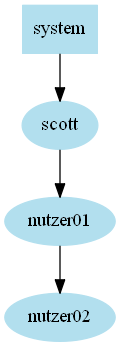
\includegraphics[scale=0.5]{Oracle_Dependency.png}
\end{center}
\subsection{Objektrechte}
Als scott:
\begin{lstlisting}[style=sql]
CREATE VIEW view2 AS
select s_name, s_vname, k_zimmer, k_server
FROM studenten, klassen
WHERE s_klasse = k_id;

GRANT SELECT ON view2 TO nutzer01 WITH GRANT OPTION;
\end{lstlisting}
Scott erstellt eine neue View view2 und erteilt nutzer01 SELECT-Rechte auf diese View, mit der Option diese Rechte weiterzugeben.

Als nutzer01:
\begin{lstlisting}[style=sql]
GRANT SELECT ON scott view2 TO nutzer02;
\end{lstlisting}
Nutzer01 gibt das SELECT-Recht an nutzer02 weiter.

Als nutzer02:
\begin{lstlisting}[style=sql]
SELECT * FROM scott view2;
\end{lstlisting}
Nutzer02 kann die Daten aus view2 anzeigen.

Als scott:
\begin{lstlisting}[style=sql]
REVOKE SELECT ON view2 FROM nutzer01;
\end{lstlisting}
Scott entzieht nutzer01 die Rechte wieder.

Als nutzer02:
\begin{lstlisting}[style=sql]
SELECT * FROM scott view2;
\end{lstlisting}
Das Statement schlägt mit folgender Fehlermeldung fehl:\\
ORA-00942: Tabelle oder View nicht vorhanden\\
Dies zeigt, das die Rechte die nutzer02 von nutzer01 erhalten hat, mit dem Entziehen der Rechte von nutzer01 durch scott kaskadierend weiter entzogend wurden.

\subsection{Systemrechte}
Als system:
\begin{lstlisting}[style=sql]
REVOKE create session FROM nutzer01;
REVOKE create session FROM nutzer02;
\end{lstlisting}
Um die Vergabe von Systemrechten zu zeigen wird nutzer01 und nutzer02 das CREATE SESSION Recht entzogen. Wenn sie sich anmelden wollen erscheint folgende Fehlermeldung:\\
ORA-01045: user STUDENT02 lacks CREATE SESSION privilege; logon denied.\\

Als system:
\begin{lstlisting}[style=sql]
GRANT create session TO nutzer01 WITH ADMIN OPTION;
\end{lstlisting}
Nutzer01 erhält das Recht wieder, diesmal mit ADMIN OPTION, damit er dieses weitergeben kann.

Als nutzer01:
\begin{lstlisting}[style=sql]
GRANT create session TO nutzer02;
\end{lstlisting}
Nutzer01 gibt das Recht an nutzer02 weiter, jetzt können sich beide Benutzer wieder anmelden.

Als system:
\begin{lstlisting}[style=sql]
REVOKE create session FROM nutzer01;
\end{lstlisting}
System einzieht nutzer01 das Recht wieder. Nutzer01 kann sich jetz nicht mehr anmelden, nutzer02 hingegen immer noch. Dies zeigt, dass Systemrechte, welche mit ADMIN OPTION weitergegeben wurden, nicht kaskadierend entzogen werden.

\section{Views}
\subsection{Rechte von Views}
Als system:
\begin{lstlisting}[style=sql]
GRANT CREATE VIEW TO nutzer01;
\end{lstlisting}
Nutzer01 erhält Rechte Views zu erstellen, damit versucht werden kann, seine SELECT-Rechte über Views weiterzugeben.

Als nutzer01:
\begin{lstlisting}[style=sql]
CREATE VIEW cheat_view AS
SELECT * FROM scott.studenten
\end{lstlisting}
Nutzer01 versucht eine View auf die geschützte Tabelle zu erstellen, dieses Statement bricht mit folgender Begründung ab:\\
ORA-01031: Nicht ausreichende Berechtigungen\\
\newpage
Als system:
\begin{lstlisting}[style=sql]
GRANT CREATE ANY VIEW TO nutzer01;
\end{lstlisting}
Nutzer01 erhält die Rechte Views auch auf fremde Tabellen zu erstellen und versucht nun, die View zu erstellen, dies bricht mit folgender Meldung ab:\\
ORA-01031: Nicht ausreichende Berechtigungen\\

Als system:
\begin{lstlisting}[style=sql]
GRANT INSERT,SELECT,UPDATE,DELETE ON scott.studenten TO nutzer01;
\end{lstlisting}
Nutzer01 erhält die Rechte nun direkt, da ihm die Rollen-Rechte nicht erlauben Views zu erstellen, er erstellt die View nun erfolgreich.

Als nutzer01:
\begin{lstlisting}[style=sql]
GRANT SELECT ON cheat_view TO nutzer02;
\end{lstlisting}
Nutzer01 gibt nun die SELECT-Rechte auf cheat\_view an nutzer02.

Als nutzer02:
\begin{lstlisting}[style=sql]
SELECT * FROM cheat_view
\end{lstlisting}
Nutzer02 versucht nun die Daten aus der View anzuzeigen, was mit folgender Meldung abbricht:\\
ORA-01720: Berechtigungsoptionen für 'SCOTT.STUDENTEN' nicht vorhanden\\
Views können also nicht verwendet werden um Rechte weiterzugeben, da diese beim ausführen der View wieder überprüft werden.

\subsection{DDL-Änderungen an den Basistabellen}
Alle Statements in diesem Absatz werden von scott durchgeführt.
\begin{lstlisting}[style=sql]
ALTER TABLE studenten ADD birthday TIMESTAMP;
\end{lstlisting}
Scott fügt eine neue Spalte birthday zu studenten hinzu.

\begin{lstlisting}[style=sql]
SELECT * FROM view1;
\end{lstlisting}
View1 kann immer noch angezeigt werden, und zeigt die gleichen Daten wie vorher an, da birthday keine der verwendeten Spalten ist.

\begin{lstlisting}[style=sql]
ALTER TABLE studenten DROP COLUMN birthday;
\end{lstlisting}
Scott entfernt die birthday Spalte wieder.

\begin{lstlisting}[style=sql]
ALTER TABLE studenten DROP COLUMN s_name;
\end{lstlisting}
Scott entfernt die s\_name spalte.

\begin{lstlisting}[style=sql]
SELECT * FROM view1;
\end{lstlisting}
View1 kann nun nicht mehr angezeigt werden, sondern das Statement bricht mit folgender Begründung ab:\\
ORA-04063: view "view1" enthält Fehler\\
Dies zeigt das Views nur von Änderungen an von ihnen verwendeten Spalten betroffen sind, da view1 s\_name verwendet. 

\begin{lstlisting}[style=sql]
ALTER TABLE studenten ADD s_name VARCHAR2(10);
\end{lstlisting}
Scott fügt s\_name wieder ein, view1 kann nun wieder angezeigt werden, enthält in s\_name nun allerdings den wert NULL.

\subsection{Updatable Views}
Alle Statements in diesem Absatz werden von scott durchgeführt.
\begin{lstlisting}[style=sql]
CREATE VIEW view_distinct AS
SELECT DISTINCT s_vname
FROM studenten;

UPDATE view_distinct SET s_vname='ana' WHERE s_vname='anna';
\end{lstlisting}
Scott erstellt eine View die alle vorkommenden Vornamen der Studenten genau einmal anzeigt.
Beim Versuch das Update-Statement auszuführen erhält scott folgende Meldung:\\
ORA-01732: Datenmanipulationsoperation auf dieser View nicht zulässig\\
Dies zeigt, das wie spezifiziert keine Daten auf Views geändert werden können die DISTINCT oder GROUP BY verwenden.

\begin{lstlisting}[style=sql]
CREATE VIEW view_all AS
SELECT *
FROM studenten
INNER JOIN klassen ON s_klassen=k_id;

UPDATE view_all SET s_name='muster' WHERE s_id=101;
\end{lstlisting}
Scott erstellt eine View, die alle Studenten mit den Informationen zu ihren klassen anzeigt. Er versucht nun mit einem Update-Statement den Namen vom Student mit der ID 101 auf 'muster' zu ändern, dies schlägt mit folgender Begründung fehl:\\
ORA-01779: Kann keine Spalte, die einer Basistabelle zugewiesen wird, verändern\\
Bei Oracle sind Daten in Views nur änderbar wenn der Schlüssel in der View auch ein Schlüssel auf der Tabelle ist. S\_id ist nicht als Schlüssel definiert.

\begin{lstlisting}[style=sql]
ALTER TABLE studenten
ADD CONSTRAINT STUDENT_PK PRIMARY KEY ( S_ID ) ENABLE;

ALTER TABLE klassen
ADD CONSTRAINT KLASSE_PK PRIMARY KEY ( K_ID ) ENABLE;
\end{lstlisting}
S\_id und k\_id werden als Primärschlüssel definiert, damit die Daten einen Schlüssel haben.

\begin{lstlisting}[style=sql]
UPDATE view_all SET s_name='muster' WHERE s_id=101;
\end{lstlisting}
Das Update kann nun erfolgreich durchgeführt werden, da s\_id sowohl ein schlüssel auf view\_all und studenten ist.

\begin{lstlisting}[style=sql]
UPDATE view_all SET k_bezeichnung='test' WHERE k_id=10;
\end{lstlisting}
Dieses Update-Statement versucht nun die Bezeichnung der Klasse mit ID 10 auf 'test' zu ändern, es schlägt mit folgender Meldung fehl:\\
ORA-01779: Kann keine Spalte, die einer Basistabelle zugewiesen wird, verändern\\
Dies liegt daran, dass eine Klasse mehreren Studenten zugewiesen sein kann, und k\_id somit kein Schlüssel vom view\_all ist.

\subsection{WITH CHECK OPTION}
\begin{lstlisting}[style=sql]
CREATE VIEW v1 AS
SELECT *
FROM studenten
WHERE s_klasse = 20 WITH CHECK OPTION;
\end{lstlisting}
Eine View v1 wird erstellt, die nur Studenten mit s\_klasse 20 ausliest und die CHECK OPTION hat.

\begin{lstlisting}[style=sql]
CREATE VIEW v2 AS
SELECT *
FROM v1
WHERE s_tel < 40000
\end{lstlisting}
Eine View v2 wird, auf Basis von v1, erstellt, die nur Studenten mit s\_tel kleiner als 40000 ausliest.

\begin{lstlisting}[style=sql]
INSERT INTO v2 VALUES (200, 'muster', 'peter', 40001, 2000, 20);
INSERT INTO v2 VALUES (201, 'muster', 'peter', 40001, 2000, 10);
\end{lstlisting}
Das erste Statement würde einen Eintrag erstellen der die Bedingungen von v1 erfüllt, die von v2 aber nicht. Das Statement wird erfolgreich durchgeführt, weil v2 keine CHECK OPTION hat.
Das zweite Statement würde einen Eintrag erstellen der die Bedingungen von v1 und v2 nicht erfüllt, es bricht mit folgender Begründung ab:\\
ORA-01402: Verletzung der WHERE-Klausel einer View WITH CHECK OPTION\\
Dies zeigt, dass die CHECK OPTION von v1 für die Bedingung von v1 immer noch gilt, auch wenn das Statement auf v2 ausgeführt wird.

\begin{lstlisting}[style=sql]
CREATE VIEW v3 AS
SELECT *
FROM v2
WHERE s_vname='peter' WITH CHECK OPTION;
\end{lstlisting}
Eine View v3 wird, auf Basis von v2, erstellt, die nur Studenten mit s\_vname peter ausliest und die CHECK OPTION hat.

\begin{lstlisting}[style=sql]
INSERT INTO v3 VALUES (202, 'muster', 'thomas', 30000, 2000, 20);
\end{lstlisting}
Dieses Statement verletzt nur die Bedingung von v3 und bricht mit folgender Meldung ab:\\
ORA-01402: Verletzung der WHERE-Klausel einer View WITH CHECK OPTION\\
Dies ist nachvollziehbar, da v3 die CHECK OPTION hat.

\begin{lstlisting}[style=sql]
INSERT INTO v3 VALUES (202, 'muster', 'peter', 30000, 2000, 20);
\end{lstlisting}
Dieses Statement verletzt keine Bedingung und wird deshalb durchgeführt.

\begin{lstlisting}[style=sql]
INSERT INTO v3 VALUES (203, 'muster', 'thomas', 30000, 2000, 10);
\end{lstlisting}
Dieses Statement verletzt nur die Bedingung von v1 und bricht mit folgender Meldung ab:\\
ORA-01402: Verletzung der WHERE-Klausel einer View WITH CHECK OPTION\\
Dies ist nicht überraschend, da schon gezeigt wurde, dass CHECK OPTION von verwendeten Views weiterhin gilt.

\begin{lstlisting}[style=sql]
INSERT INTO v3 VALUES (204, 'muster', 'thomas', 40000, 2000, 20);
\end{lstlisting}
Dieses Statement verletzt nur die Bedingung von v2 und bricht mit folgender Meldung ab:\\
ORA-01402: Verletzung der WHERE-Klausel einer View WITH CHECK OPTION\\
Dies zeigt, dass die CHECK OPTION von v3 sich somit auf alle Bedingungen von verwendeten Views bezieht und egal ist, ob diese selber CHECK OPTION haben.
\chapter{MS SQL Express 2012}
\section{Vorbereitung}
Dieser Teil der Ausarbeitung wurde auf einem MS SQL Server Express 2012 auf einem Windows 7 Notebook durchgeführt. Um die User nicht auf dem Server und der Datenbank zu erstellen wurde die Datenbank dbarc03 als partial contained Datenbank erstellt, dafür musste dies zuerst aktiviert werden:
\begin{lstlisting}[style=sql]
SP_CONFIGURE 'show advanced options',1;
RECONFIGURE;
GO;
SP_CONFIGURE 'contained database authentication',1;
RECONFIGURE;
GO;
SP_CONFIGURE 'show advanced options',0;
RECONFIGURE;
GO;
\end{lstlisting}
\subsection{Einrichten User}
Als sytem:
\begin{lstlisting}[style=sql]
CREATE USER scott WITH PASSWORD = 'tiger';
CREATE USER nutzer01 WITH PASSWORD = 'nutzer01';
CREATE USER nutzer02 WITH PASSWORD = 'nutzer02';

GRANT CREATE ROLE TO scott;
GRANT CREATE VIEW TO scott;
GRANT CREATE TABLE TO scott;
GRANT CONTROL ON SCHEMA :: dbo TO scott;
\end{lstlisting}
Es werden die User scott, nutzer01 und nutzer02 analog zu der Durchführung in Oracle erstellt, CREATE SESSION Rechte sind in MS SQL nicht nötig um sich anzumelden. Scott erhält für das folgende Vorgehen Rechte um Rollen, Tabellen und Views zu erstellen, zusätzlich benötigt er noch Rechte um das Schema dbo zu verwalten.
\newpage
\section{Zugriffssteuerung mit User und Rollen}
\subsection{Tabellen erzeugen}
Als scott:
\begin{lstlisting}[style=sql]
CREATE TABLE klassen(
k_id INTEGER,
k_bezeichnung VARCHAR(20),
k_zimmer VARCHAR(10),
k_server VARCHAR(10));

CREATE TABLE studenten(
s_id INTEGER,
s_name VARCHAR(10),
s_vname VARCHAR(10),
s_tel VARCHAR(20),
s_konto_stand INTEGER,
s_klasse INTEGER);


INSERT INTO klassen values ( 10, 'ia00', '3333' , 'pluto');
INSERT INTO klassen values ( 20, 'ia01', '2222' , 'saturn');

INSERT INTO studenten values( 101, 'meier', 'hans', '11111', 5000, 10);
INSERT INTO studenten values( 102, 'hirt', 'otto', '22222', -100, 10);
INSERT INTO studenten values( 103, 'kok', 'thomas', '33333', 1000, 20);
INSERT INTO studenten values( 104, 'guzman', 'anna', '44444', 3000, 20);
INSERT INTO studenten values( 105, 'lorch', 'felix', '45678', 7000, 20);
\end{lstlisting}
Die Tabellen werden analog zur Oracle Übung erstellt, der Datentyp NUMBER(9) wurde durch INTEGER ersetzt und VARCHAR2 durch VARCHAR, da diese Typen unter MS SQL nicht existieren.
\subsection{View erstellen}
Als scott:
\begin{lstlisting}[style=sql]
CREATE VIEW view1 AS
select s_name, s_vname, k_zimmer, k_server
FROM studenten, klassen
WHERE s_klasse = k_id
\end{lstlisting}
Scott erstellt eine View view1 in der Daten aus studenten und klassen angezeigt werden.

\subsection{Rollen definieren}
Als scott:
\begin{lstlisting}[style=sql]
CREATE ROLE view1_verwalter;
CREATE ROLE view1_nutzer;
\end{lstlisting}
Scott erstellt die Rollen view1\_verwalter und view1\_nutzer.
\newpage
\subsection{Den Rollen Rechte zuweisen}
Als scott:
\begin{lstlisting}[style=sql]
GRANT INSERT,SELECT,UPDATE,DELETE ON studenten TO view1_verwalter;
GRANT INSERT,SELECT,UPDATE,DELETE ON klassen TO view1_verwalter;
\end{lstlisting}
Scott erteilt der Rolle view1\_verwalter die Rechte Daten in studenten und klassen zu sehen und zu verändern.

Als scott:
\begin{lstlisting}[style=sql]
GRANT SELECT ON view1 TO view1_nutzer;
\end{lstlisting}
Scott erteilt der Rolle view1\_nutzer das Recht die Daten in view1 zu lesen.

\subsection{Den User Rollen zuweisen}
Als scott:
\begin{lstlisting}[style=sql]
GRANT view1_verwalter TO nutzer01;
GRANT view1_nutzer TO nutzer02;
\end{lstlisting}
Scott weist nutzer01 die Rolle view1\_verwalter und nutzer02 die Rolle view2\_nutzer zu.

\subsection{Überprüfung der Rechte der beiden Rollen}
Die folgenden Statements werden zur Überprüfung der Rechte verwendet:
\begin{lstlisting}[style=sql]
SELECT * FROM scott.studenten;
INSERT INTO scott.studenten VALUES (106, 'peter', 'muster', 12345,2000,20);
UPDATE scott.studenten SET s_tel = 54321 WHERE s_id = 106;
DELETE FROM scott.studenten WHERE s_id = 106;

SELECT * FROM scott.klassen;
INSERT INTO scott.klassen VALUES (30, 'ia02', 1111, 'uranus');
UPDATE scott.klassen SET k_zimmer = 4444 WHERE k_id = 30;
DELETE FROM scott.klassen WHERE k_id = 30;

SELECT * FROM scott.view1;
INSERT INTO scott.view1 VALUES ('peter','muster',2222,'saturn');
UPDATE scott.view1 SET s_name = 'kook' WHERE s_vname = 'thomas';
DELETE FROM scott.view1 WHERE s_vname = 'thomas';
\end{lstlisting}
\subsubsection{Was kann der Verwalter lesen und bearbeiten?}
Die Statements in den Linien 1 bis 9 können von nutzer01 ausgeführt werden. Wenn nutzer01 das Statement in Linie 11 ausführen will erhält er folgende Fehlermeldung:\\
The SELECT permission was denied on the object 'view1', database 'dbarc03', schema 'dbo'.\\
Im Gegensatz zu Oracle bestätigt MS SQL somit, das die View existiert. Bei den Statements in Linie 12 bis 14 erhält nutzer01 folgende Meldung:\\
View or function 'view1' is not updatable because the modification affects multiple base tables.\\
MS SQL wertet hier also die Gültigkeit des Statements vor den Berechtigungen aus, was dazu führt das nutzer01 Informationen über gültige Statements auf view1 erhält, obwohl er keinen Zugriff darauf hat, abgesehen von den Meldungen funktioniert das Berechtigungskonzept hier analog zu Oracle.
\subsubsection{Was kann der Nutzer lesen und bearbeiten?}
Wenn nutzer02 die Statements in den Linien 1 bis 9 durchführen will erhält er folgende Meldungen:\\
The SELECT permission was denied on the object 'klassen', database 'dbarc03', schema 'dbo'.\\
The SELECT permission was denied on the object 'studenten', database 'dbarc03', schema 'dbo'.\\
Auch hier zeigt MS SQL das die Tabellen zwar vorhanden sind, nutzer02 aber keine Berechtigungen hat. Nutzer02 kann das Statement in Linie 11 ausführen, bei den Statements in Linien 12 bis 14 erhält er auch folgende Meldung:\\
View or function 'view1' is not updatable because the modification affects multiple base tables.\\
Auch hier wird die Gültigkeit vor den Berechtigungen ausgewertet, die Berechtigungen funktionieren aber auch analog zu Oracle.
\section{Zugriffsrechte: Objekt- und Systemrechte}
\begin{center}
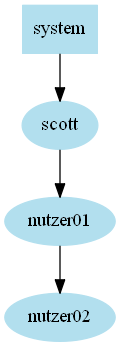
\includegraphics[scale=0.5]{Oracle_Dependency.png}
\end{center}
\subsection{Objektrechte}
Als scott:
\begin{lstlisting}[style=sql]
CREATE VIEW view2 AS
select s_name, s_vname, k_zimmer, k_server
FROM studenten, klassen
WHERE s_klasse = k_id;

GRANT SELECT ON view2 TO nutzer01 WITH GRANT OPTION;
\end{lstlisting}
Scott erstellt eine View view2 und erteilt nutzer01 das SELECT-Recht dazu, mit der Option dieses weiterzugeben.

Als nutzer01:
\begin{lstlisting}[style=sql]
GRANT SELECT ON view2 TO nutzer02;
\end{lstlisting}
Nutzer01 gibt das SELECT-Recht an nutzer02 weiter.

Als nutzer02:
\begin{lstlisting}[style=sql]
SELECT * FROM scott view2;
\end{lstlisting}
Nutzer02 kann die Daten aus view2 erfolgreich weitergeben.
\newpage
Als scott:
\begin{lstlisting}[style=sql]
REVOKE SELECT ON view2 FROM nutzer01 CASCADE;
\end{lstlisting}
Scott entzieht nutzer01 die Rechte auf view2 wieder, das Schlüsselwort CASCADE muss bei MS SQL angegeben werden, sobald Rechte mit WITH GRANT OPTION erteilt wurden, auch wenn diese noch nicht weiter gegeben wurden, ansonsten bricht das REVOKE-Statement mit folgender Meldung ab:\\
To revoke or deny grantable privileges, specify the CASCADE option.

Als nutzer02:
\begin{lstlisting}[style=sql]
SELECT * FROM scott view2;
\end{lstlisting}
Das Statement schlägt mit folgender Meldung fehl:\\
The SELECT permission was denied on the object 'view2', database 'dbarc03', schema 'dbo'.\\
Die Berechtigungen wurden also, wie das Schlüsselwort CASCADE impliziert, kaskadierend entzogen, MS SQL schützt also davor, Rechte unbewusst kaskadierend zu entziehen.

\subsection{Systemrechte}
Als system:
\begin{lstlisting}[style=sql]
GRANT CREATE VIEW TO nutzer01 WITH GRANT OPTION;
\end{lstlisting}
Nutzer01 werden die Rechte erteilt, eine View zu erstellen mit der Option dieses Recht weiterzugeben. Da MS SQL das WITH ADMIN OPTION nicht kennt muss hier auch WITH GRANT OPTION verwendet werden.

als nutzer01:
\begin{lstlisting}[style=sql]
GRANT CREATE VIEW TO nutzer02;
\end{lstlisting}
Nutzer01 gibt das Recht an nutzer02 weiter.

Als system:
\begin{lstlisting}[style=sql]
REVOKE CREATE VIEW FROM nutzer01 CASCADE;
\end{lstlisting}
Da das Recht wieder mit GRANT OPTION weitergegeben wurde, muss auch hier beim entfernen das Schlüsselwort CASCADE angegeben werden, und Systemrechte werden dadurch, im Gegensatz zu Oracle, kaskadierend entzogen.

\section{Views}
\subsection{Rechte von Views}
Als system:
\begin{lstlisting}[style=sql]
GRANT CREATE VIEW TO nutzer01;
GRANT ALTER ON SCHEMA :: dbo TO nutzer01;
\end{lstlisting}
Nutzer01 wird das Recht Views zu erstellen erteilt, gleichzeitig benötigt er auch das Recht, das Schema dbo zu ändern.
\newpage
Als nutzer01:
\begin{lstlisting}[style=sql]
CREATE VIEW cheat_view AS
SELECT * FROM studenten;
\end{lstlisting}
Nutzer01 kann die View nun erstellen, was unter Oracle nicht ging, dies liegt an der ALTER Berechtigung auf dbo.
Als nutzer01:
\begin{lstlisting}[style=sql]
SELECT * FROM cheat_view
\end{lstlisting}
Nutzer01 versucht nun die Daten der eben erstellten view anzuzeigen, dies schlägt mit folgender Meldung fehl:\\
The SELECT permission was denied on the object 'cheat\_view', database 'dbarc03', schema 'dbo'.\\
Dies zeigt, dass nutzer01 keine Berechtigungen hat Views von dbo anzuzeigen, auf die er nicht explizit Berechtigungen hat.

Als nutzer01:
\begin{lstlisting}[style=sql]
DROP VIEW cheat_view;
\end{lstlisting}
Nutzer01 löscht die View wieder.

Als system:
\begin{lstlisting}[style=sql]
CREATE SCHEMA nutzer01 AUTHORIZATION nutzer01;
\end{lstlisting}
Nutzer01 erhält sein eigenes Schema, auf dem er volle Berechtigungen hat.

Als nutzer01:
\begin{lstlisting}[style=sql]
CREATE VIEW nutzer01.cheat_view AS
SELECT * FROM dbo.studenten;
\end{lstlisting}
Nutzer01 erstellt die View im nutzer01 Schema.

Als nutzer01:
\begin{lstlisting}[style=sql]
SELECT * FROM nutzer01.cheat_view;
GRANT SELECT ON nutzer01.cheat_view TO nutzer02;
\end{lstlisting}
Nutzer01 kann die View nun selber erfolgreich anzeigen, er gibt die SELECT-Rechte an nutzer02 weiter, welcher die Daten ja nicht sehen dürfte.

Als nutzer02:
\begin{lstlisting}[style=sql]
SELECT * FROM nutzer01.cheat_view
\end{lstlisting}
Nutzer02 versucht nun die Daten auszulesen, was mit folgender Meldung abbricht:\\
The SELECT permission was denied on the object 'studenten', database 'dbarc03', schema 'dbo'.\\
Diese Meldung zeigt eindeutig, das die Rechte auf dbo fehlen, und nicht auf nutzer01, auch bei MS SQL können Views also nicht verwendet werden, um Berechtigungen unerlaubt weiterzugeben.
\newpage
\subsection{DDL-Änderungen an den Basistabellen}
Alle Statements in folgendem Absatz werden als scott durchgeführt.
\begin{lstlisting}[style=sql]
ALTER TABLE studenten ADD birthday TIMESTAMP;
\end{lstlisting}
Scott fügt eine Spalte brithday zu studenten hinzu.

\begin{lstlisting}[style=sql]
SELECT * FROM view1;
\end{lstlisting}
View1 lässt sich immer noch unverändert abrufen, da birhday von ihr nicht abgefragt wird.

\begin{lstlisting}[style=sql]
ALTER TABLE studenten DROP COLUMN birthday;
\end{lstlisting}
Scott entfernt birthday wieder.

\begin{lstlisting}[style=sql]
ALTER TABLE studenten DROP COLUMN s_name;
\end{lstlisting}
Scott entfernt die Spalte s\_name.

\begin{lstlisting}[style=sql]
SELECT * FROM view1;
\end{lstlisting}
View1 kann nun nicht mehr angezeigt werden, sondern bricht mit folgender Meldung ab:\\
Invalid column name 's\_name'.
Could not use view or function 'view1' because of binding errors.\\
Dies zeigt, das auch unter MS SQL nur Spalten, welche auch verwendet werden, die View beeinflussen.

\begin{lstlisting}[style=sql]
ALTER TABLE studenten ADD s_name VARCHAR(10);
\end{lstlisting}
Scott fügt die Spale wieder ein, view1 kann wieder angezeigt werden, enthält jetzt aber NULL in s\_name.

\subsection{Updatable Views}
Alle Statements in folgendem Absatz werden als scott durchgeführt.
\begin{lstlisting}[style=sql]
CREATE VIEW view_distinct AS
SELECT DISTINCT s_vname
FROM studenten;

UPDATE view_distinct SET s_vname='ana' WHERE s_vname='anna';
\end{lstlisting}
Scott erstellt eine View, welche das Schlüsselwort DISTINCE verwendet, und versucht ein UPDATE-Statement auzuführen, was abbricht:\\
Cannot update the view or function 'view\_distinct' because it contains aggregates, or a DISTINCT or GROUP BY clause, or PIVOT or UNPIVOT operator.\\
Die Meldung beschreibt sehr ausführlich, welche Schlüsselwörter dazu führen, dass über eine View keine Daten verändert werden können.

\begin{lstlisting}[style=sql]
CREATE VIEW view_all AS
SELECT *
FROM studenten
INNER JOIN klassen ON s_klasse=k_id;
\end{lstlisting}
\newpage
Scott erstellt nun eine View view\_all die alle Daten der Studenten und ihren Klassen anzeigt.

\begin{lstlisting}[style=sql]
UPDATE view_all SET s_name='muster' WHERE s_id=101;
\end{lstlisting}
Scott versucht nun den Namen des Studenten 101 über die View zu ändern, dies ist im Gegensatz zu Oracle möglich, obwohl keine Schlüssel definiert sind.

\begin{lstlisting}[style=sql]
UPDATE view_all SET k_zimmer=4444 WHERE k_id=20;
\end{lstlisting}
Scott versucht nun das Zimmer der Klasse 20 über die View zu ändern, 
auch dies funktioniert, obwohl die Klasse 20 mehrmals vorkommt, MS SQL kennt folglich keinen Schutz wie Oracle.

\subsection{WITH CHECK OPTION}
\begin{lstlisting}[style=sql]
CREATE VIEW v1 AS
SELECT *
FROM studenten
WHERE s_klasse = 20 WITH CHECK OPTION;
\end{lstlisting}
Scott erstellt eine View v1 die alle Studenten aus Klasse 20 anzeigt, und definiert die CHECK OPTION.

\begin{lstlisting}[style=sql]
CREATE VIEW v2 AS
SELECT *
FROM v1
WHERE s_tel < 40000
\end{lstlisting}
Scott erstellt eine View v2, basierend auf v2, die nur Einträge mit s\_tel kleiner als 40000 anzeigt.

\begin{lstlisting}[style=sql]
INSERT INTO v2 VALUES (200, 'muster', 'peter', 40001, 2000, 20);
INSERT INTO v2 VALUES (201, 'muster', 'peter', 40001, 2000, 10);
\end{lstlisting}
Das erste Statement wird ausgeführt, da es nur die Bedingung der View ohne CHECK OPTION verletzt. Das zweite Statement bricht mit folgender Begründung ab:\\
The attempted insert or update failed because the target view either specifies WITH CHECK OPTION or spans a view that specifies WITH CHECK OPTION and one or more rows resulting from the operation did not qualify under the CHECK OPTION constraint.\\
Die CHECK OPTION betrifft also wie in Oracle die Bedingung von v2 nicht.

\begin{lstlisting}[style=sql]
CREATE VIEW v3 AS
SELECT *
FROM v2
WHERE s_vname='peter' WITH CHECK OPTION;
\end{lstlisting}
Scott erstellt eine View v3, basierend auf v2, mit der Bedingung das der Vorname peter ist und der CHECK OPTION.

\begin{lstlisting}[style=sql]
INSERT INTO v3 VALUES (202, 'muster', 'thomas', 30000, 2000, 20);
\end{lstlisting}
Da dieses Statement  die Bedingung von v3 verletzt, bricht es mit folgender Meldung ab:\\
The attempted insert or update failed because the target view either specifies WITH CHECK OPTION or spans a view that specifies WITH CHECK OPTION and one or more rows resulting from the operation did not qualify under the CHECK OPTION constraint.\\

\begin{lstlisting}[style=sql]
INSERT INTO v3 VALUES (202, 'muster', 'peter', 30000, 2000, 20);
\end{lstlisting}
Dieses Statement verletzt keine Bedingungen und läuft durch.

\begin{lstlisting}[style=sql]
INSERT INTO v3 VALUES (203, 'muster', 'peter', 30000, 2000, 10);
\end{lstlisting}
Da dieses Statement  die Bedingung von v1 verletzt, bricht es mit folgender Meldung ab:\\
The attempted insert or update failed because the target view either specifies WITH CHECK OPTION or spans a view that specifies WITH CHECK OPTION and one or more rows resulting from the operation did not qualify under the CHECK OPTION constraint.\\


\begin{lstlisting}[style=sql]
INSERT INTO v3 VALUES (204, 'muster', 'peter', 40000, 2000, 20);
\end{lstlisting}
Da dieses Statement  die Bedingung von v2 verletzt, bricht es mit folgender Meldung ab:\\
The attempted insert or update failed because the target view either specifies WITH CHECK OPTION or spans a view that specifies WITH CHECK OPTION and one or more rows resulting from the operation did not qualify under the CHECK OPTION constraint.\\
Die CHECK OPTION hat also wie bei Oracle auch unter MS SQL den Effekt, das Bedingungen von verwendeten Views auch geprüft werden, wenn nur die verwendende View die CHECK OPTION gesetzt hat.

\chapter{MySQL}
Für diese Ausarbeitung verwenden wir XAMPP 1.7.3 mit MySQL 5.5.27.
\section{Vorbereitung}
\subsection{Einrichtung User}
\begin{lstlisting}[style=sql]
CREATE USER scott@localhost IDENTIFIED BY 'tiger';
CREATE USER nutzer01@localhost IDENTIFIED BY 'nutzer01';
CREATE USER nutzer02@localhost IDENTIFIED BY 'nutzer02';
GRANT ALL PRIVILEGES ON `dbarc03` . * TO 'scott'@'localhost';
\end{lstlisting}
Bei MySQL muss bei der Erstellung von Benutzern neben dem Namen und der Identifizierungsmethode auch definiert werden vom welchem Server aus sich der Nutzereinloggen darf. Da unser MySQL Server lokal läuft, wird hier 'localhost' angegeben. Daneben gibt es auch IP und Servername, sowie die Berechtigung ohne Einschränkungen (\%) und die Regelung der Zugriffe per Hosttabelle.
\subsection{Einrichtung Datenbank}
\begin{lstlisting}[style=sql]
CREATE DATABASE dbarc03;
\end{lstlisting}

\section{Zugriffssteuerung mit User und Rollen}
\subsection{Tabellen erzeugen}
Als Benutzer 'scott':
\begin{lstlisting}[style=sql]
CREATE TABLE studenten(
s_id int(9) PRIMARY KEY,
s_name VARCHAR(10),
s_vname VARCHAR(10),
s_tel VARCHAR(20),
s_konto_stand int(9),
s_klasse int(9));

CREATE TABLE klassen(
k_id int(9),
k_bezeichnung VARCHAR(20),
k_zimmer VARCHAR(10),
k_server VARCHAR(10));

INSERT INTO klassen values( 10, 'ia00', '3333' , 'pluto');
INSERT INTO klassen values( 20, 'ia01', '2222' , 'saturn');

INSERT INTO studenten values( 101, 'meier', 'hans', '11111', 5000, 10);
INSERT INTO studenten values( 102, 'hirt', 'otto', '22222', -100, 10);
INSERT INTO studenten values( 103, 'kok', 'thomas', '33333', 1000, 20);
INSERT INTO studenten values( 104, 'guzman', 'anna', '44444', 3000, 20);
INSERT INTO studenten values( 105, 'lorch', 'felix', '45678', 7000, 20);
\end{lstlisting}

\subsection{View erstellen}
\begin{lstlisting}[style=sql]
CREATE VIEW view1 AS
SELECT s_name, s_vname, k_zimmer, k_server
FROM studenten, klassen
WHERE s_klasse = k_id
\end{lstlisting}

\subsection{Rechte an User verteilen}
Als 'root':
\begin{lstlisting}[style=sql]
REVOKE ALL PRIVILEGES ON `dbarc03` . * FROM scott@localhost;
GRANT SELECT, INSERT, UPDATE, DELETE, CREATE, DROP, INDEX, ALTER, CREATE
VIEW, SHOW VIEW
ON `dbarc03` . *
TO scott@localhost WITH GRANT OPTION;
\end{lstlisting}
Scott kann nun seine Rechte frei weitergeben.

Als Benutzer 'scott':
\begin{lstlisting}[style=sql]
GRANT SELECT, INSERT, UPDATE, DELETE ON studenten TO
nutzer01@localhost;

GRANT SELECT, INSERT, UPDATE, DELETE ON klassen TO
nutzer01@localhost;

GRANT SELECT ON view1 TO nutzer02@localhost;
\end{lstlisting}
In MySQL gibt es, im Gegensatz zu Oracle, keine Rollen. Man muss also jedem Nutzer die Rechte direkt zuteilen.\newline
Deswegen gibt hier 'scott' dem Benutzer 'nutzer01' select-, insert-, update- und delete-Rechte für die beiden Tabellen 'studenten' und 'klassen' und dem Benutzer 'nutzer02' select-Rechte an der View 'view1'.\newline\newline

\subsection{Überprüfung der Rechte der beiden Nutzer}
\Bold{Statement 1}
\begin{lstlisting}[style=sql]
SELECT * FROM dbarc03.studenten;
INSERT INTO dbarc03.studenten VALUES (106, 'peter', 'muster', 12345,2000,20);
UPDATE dbarc03.studenten SET s_tel = 54321 WHERE s_id = 106;
DELETE FROM dbarc03.studenten WHERE s_id = 106;
\end{lstlisting}
\Bold{Statement 2}
\begin{lstlisting}[style=sql]
SELECT * FROM dbarc03.klassen;
INSERT INTO dbarc03.klassen VALUES (30, 'ia02', 1111, 'uranus');
UPDATE dbarc03.klassen SET k_zimmer = 4444 WHERE k_id = 30;
DELETE FROM dbarc03.klassen WHERE k_id = 30;
\end{lstlisting}
\newpage
\Bold{Statement 3}
\begin{lstlisting}[style=sql]
SELECT * FROM dbarc03.view1;
INSERT INTO dbarc03.view1 VALUES ('peter','muster',2222,'saturn');
UPDATE dbarc03.view1 SET s_name = 'kook' WHERE s_vname = 'thomas';
DELETE FROM dbarc03.view1 WHERE s_vname = 'thomas';
\end{lstlisting}
Die obigen 3 Statements werden jeweils von 'nutzer01' und 'nutzer02' ausgeführt.
\subsubsection{Was kann nutzer01 lesen und bearbeiten?}
'nutzer01' kann die ersten beiden Statements ausführen. Er kann also Daten der beiden Tabellen 'studenten' und 'klassen' auslesen, ergänzen, verändern und löschen. Er kann keinerlei Operationen auf der View 'view1' ausführen. Dies verhält sich also wie bei Oracle.
\subsubsection{Was kann nutzer02 lesen und bearbeiten?}
Im Gegensatz zu 'nutzer01' kann 'nutzer02' keinerlei Operationen an den Tabellen 'studenten' und 'klassen' durchführen. Wie erwartet kann er in Statement 3 die Daten aus der View 'view1' lediglich auslesen. Auch hier verhält sich MySQL genauso wie bei Oracle.

\section{Zugriffsrechte: Objekt- und Systemrechte}
\begin{center}
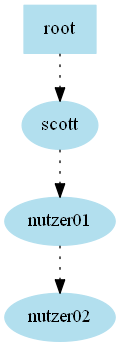
\includegraphics[scale=0.5]{MySQL_Dependency.png}
\end{center}
\Bold{Berechtigungen unter MySQL}\newline
Berechtigungen werden unter MySQL in 4 Stufen klassifiziert:\newline\newline
\Bold{Globale Ebene}\newline
Globale Rechte gelten für alle Datenbanken auf einem bestimmten Server und werden in der Systemtabelle mysql.user gespeichert\newline
\Bold{Datenbankebene}\newline
Datenbankrechte gelten für alle Tabellen einer bestimmten Datenbank und werden in der Systemtabelle mysql.db gespeichert\newline
\Bold{Tabellenebene}\newline
Tabellenrechte gelten für alle Spalten einer bestimmten Tabelle und werden in der Systemtabelle mysql.tables\_priv gespeichert\newline
\Bold{Spaltenebene}\newline
Spaltenrechte gelten für einzelne Spalten einer bestimmtem Tabelle und werden in der Systembtabelle mysql.columns\_priv gespeichert
\newline\newline\small{Quelle: 'SQL in a Nutshell' by Kevin E. Klinke, 2.Auflage, S: 307}
\subsection{Objektrechte}
Um die Objektrechte überprüfen zu können erstellen wir als Benutzer 'scott' eine zweite View namens 'view2'. Wir geben 'nutzer01' select-Rechte für diese View.
\begin{lstlisting}[style=sql]
CREATE VIEW view2 AS
select s_name, s_vname, k_zimmer, k_server
FROM studenten, klassen
WHERE s_klasse = k_id;

GRANT SELECT ON dbarc03.view2 TO nutzer01@localhost WITH GRANT OPTION;
\end{lstlisting}

'nutzer01' gibt diese select-Rechte an der View 'view2' nun weiter an 'nutzer02'.
\begin{lstlisting}[style=sql]
GRANT SELECT ON dbarc03.view2 TO nutzer02@localhost;
\end{lstlisting}

'nutzer02' testet, ob er nun das Recht hat Daten aus 'view2' auszulesen.
\begin{lstlisting}[style=sql]
SELECT * FROM dbarc03.view2;
\end{lstlisting}
Erfolgreich.

Nun nimmt 'scott' die selec-Rechte an der View 'view2' dem Nutzer 'nutzer01' wieder weg.
\begin{lstlisting}[style=sql]
REVOKE SELECT ON dbarc03.view2 FROM nutzer01@localhost;
\end{lstlisting}

Anschliessend testen wir als 'nutzer02' ob wir immernoch select-Rechte auf 'view2' haben oder ob diese mit dem Entfernen der Rechte von 'nutzer01' ebenfalls erloschen sind. 
\begin{lstlisting}[style=sql]
SELECT * FROM dbarc03.view2;
\end{lstlisting}
Immernoch erfolgreich.
\newline\newline
MySQL verhält sich hier grundlegend anders als Oracle. Es gibt zwei Arten einem Nutzer Rechte zu geben. Mit 'WITH GRANT OPTION' oder ohne.\newline
Ohne 'WITH GRANT OPTION' können die Rechte nicht weitergegeben werden. Mit 'WITH GRANT OPTION' können Rechte uneingeschränkt weitergegeben werden. Anders als bei Oracle entstehen so keine Abhängigkeiten und somit keine Kaskadeneffekte.
\newpage
\subsection{Systemrechte}
Um die Systemrechte zu überprüfen erhält Nutzer 'scott' das Recht neue Nutzer zu erstellen.
\begin{lstlisting}[style=sql]
GRANT CREATE USER ON *.* TO scott@localhost WITH GRANT OPTION;
\end{lstlisting}

'scott' gibt dieses Recht anschliessen an 'nutzer01' weiter.
\begin{lstlisting}[style=sql]
GRANT CREATE USER ON *.* TO nutzer01@localhost;
\end{lstlisting}

Nun entzieht der Root 'scott' das Recht neue Nutzer zu erstellen wieder.
\begin{lstlisting}[style=sql]
REVOKE CREATE USER ON *.* FROM scott@localhost;
\end{lstlisting}

'nutzer01' testet ob er immernoch neue Nutzer erstellen kann.
\begin{lstlisting}[style=sql]
CREATE USER test@localhost IDENTIFIED BY 'test';
\end{lstlisting}
Erfolgreich.
\newline\newline
Auch hier entsteht keine Kaskade. In MySQL verhalten sich Objekt- und Systemrechte identisch.

\section{Views}
\subsection{Rechte von Views}
Zuerst erhält 'nutzer01' das Recht neue Views zu erstellen.
\begin{lstlisting}[style=sql]
GRANT CREATE VIEW ON `dbarc03` .* TO nutzer01@localhost;
\end{lstlisting}

'nutzer01' erstellt hierauf die View 'cheat\_view' auf die Daten in der Tabelle 'studenten'.
\begin{lstlisting}[style=sql]
CREATE VIEW cheat_view AS
SELECT * FROM dbarc03.studenten;
\end{lstlisting}
Erfolgreich.

'nutzer01' gibt nun 'nutzer02' das select-Recht für die View 'cheat\_view'.
\begin{lstlisting}[style=sql]
GRANT SELECT ON cheat_view TO nutzer02@localhost;
\end{lstlisting}
Error Code: 1142. SELECT command denied to user 'nutzer01'@'localhost' for table 'cheat\_view'\newline\newline
In MySQL wird die View, welche 'nutzer01' erstellt hat, nicht in einem Tablespace gespeichert, welcher 'nutzer01' gehört. Folglich hat er keinerlei Rechte auf der von ihm erstellten View und kann diese so natürlich auch nicht weitergeben.
\newpage
\subsection{DDL-Änderungen an den Basistabellen}
Erst überprüfen wir wie sich die View 'view1' verhält, wenn der Nutzer 'scott' die Tabelle 'studenten' um eine Spalte 'birthday' erweitert.
\begin{lstlisting}[style=sql]
ALTER TABLE studenten ADD birthday TIMESTAMP;
\end{lstlisting}

\begin{lstlisting}[style=sql]
SELECT * FROM view1;
\end{lstlisting}
Es entstehen keinerlei Probleme, da 'view1' durch die neu Spalte nicht beeinträchtigt wird.\newline\newline

Als nächstes löscht 'scott' die soeben erstellte Spalte 'birthday' wieder aus der Tabelle 'studenten', zusammen mit der vorhandenen Spalte 's\_name'.
\begin{lstlisting}[style=sql]
ALTER TABLE studenten DROP COLUMN birthday;
ALTER TABLE studenten DROP COLUMN s_name;
\end{lstlisting}

\begin{lstlisting}[style=sql]
SELECT * FROM view1;
\end{lstlisting}
Error Code: 1356. View 'dbarc03.view1' references invalid table(s) or column(s) or function(s) or definer/invoker of view lack rights to use them\newline\newline
Wie man aus der Fehlermeldung erkennen kann, referenziert 'view1' immernoch auf die soeben gelöschte Spalte 's\_name'.\newline\newline

Wir fügen die Spalte 's\_name' wieder hinzu um so die View 'view1' wieder zu 'reparieren'.
\begin{lstlisting}[style=sql]
ALTER TABLE studenten ADD s_name VARCHAR(10);
\end{lstlisting}

\subsection{Updatable Views}
Nun wollen wir überprüfen was passiert, wenn man versucht über eine View die Daten der Tabelle zu verändern.\newline\newline

Nutzer 'scott' erstellt hierfür eine neue View 'view\_distinct'. Anschliessend versucht er die Daten der Spalte 's\_vname' via update-Statement zu verändern.
\begin{lstlisting}[style=sql]
CREATE VIEW view_distinct AS
SELECT DISTINCT s_vname
FROM studenten;

UPDATE view_distinct SET s_vname='ana' WHERE s_vname='anna';
\end{lstlisting}
Error Code: 1288. The target table view\_distinct of the UPDATE is not updatable\newline\newline
MySQL verhält sich genauso wie Oracle.\newline\newline

Anschliessend erstellt 'scott' eine weitere View 'view\_all', diesmal ohne distinct.
\begin{lstlisting}[style=sql]
CREATE VIEW view_all AS
SELECT *
FROM studenten
INNER JOIN klassen ON s_klasse=k_id;
\end{lstlisting}
'scott' versucht nun die Daten der Tabelle über ein update-Statement auf 'view\_all' zu verändern.
\begin{lstlisting}[style=sql]
SELECT * FROM view_all;

UPDATE view_all SET s_name='muster' WHERE s_id=101;
\end{lstlisting}
Dies gelingt, wie bei Oracle.

\begin{lstlisting}[style=sql]
UPDATE view_all SET k_bezeichnung='test' WHERE k_id=10;
\end{lstlisting}

\subsection{WITH CHECK OPTION}
Die \Bold{WITH CHECK OPTION}-Klausel kann für eine veränderbare View benutzt werden, um Einfügungen oder Änderungen an Zeilen zu verhindern, welche die \Bold{WHERE}-Klausel des SELECT-Statements nicht erfüllen.
In einer \Bold{WITH CHECK OPTION}-Klausel einer veränderbaren View legen die Schlüsselwörter \Bold{LOCAL} und \Bold{CASCADED} den Rahmen der Überprüfungen fest, wenn die View auf Grundlage einer anderen View definiert wurde. Das Schlüsselwort \Bold{LOCAL} schränkt die \Bold{CHECK OPTION} auf die View ein, die gerade definiert wird, während \Bold{CASCADED} dafür sorgt, dass sich die Prüfungen auch auf die zugrunde liegenden Views erstrecken. Wenn keines der beiden Schlüsselwörter angegeben ist, ist \Bold{CASCADED} der Standard.\newline\newline
\small{Quelle: http://dev.mysql.com/doc/refman/5.1/de/create-view.html}\newline\newline

Nun wollen wir das Verhalten von \Bold{WITH CHECK OPTION} in MySQL untersuchen.
\begin{lstlisting}[style=sql]
CREATE VIEW v1 AS
SELECT *
FROM studenten
WHERE s_klasse = 20 WITH CHECK OPTION;
\end{lstlisting}

\begin{lstlisting}[style=sql]
CREATE VIEW v2 AS
SELECT *
FROM v1
WHERE s_tel < 40000
\end{lstlisting}

\begin{lstlisting}[style=sql]
INSERT INTO v2 VALUES (200, 'muster', 'peter', 40001, 2000, 20);
INSERT INTO v2 VALUES (201, 'muster', 'peter', 40001, 2000, 10);
\end{lstlisting}
Erfolgreich.

\begin{lstlisting}[style=sql]
CREATE VIEW v3 AS
SELECT *
FROM v2
WHERE s_vname='peter' WITH CHECK OPTION;
\end{lstlisting}

\begin{lstlisting}[style=sql]
INSERT INTO v3 VALUES (202, 'muster', 'thomas', 30000, 2000, 20);
\end{lstlisting}
Error Code: 1369. CHECK OPTION failed 'dbarc03.v3'

\begin{lstlisting}[style=sql]
INSERT INTO v3 VALUES (202, 'muster', 'peter', 30000, 2000, 20);
\end{lstlisting}
Error Code: 1369. CHECK OPTION failed 'dbarc03.v3'
\newpage
\begin{lstlisting}[style=sql]
INSERT INTO v3 VALUES (203, 'muster', 'thomas', 30000, 2000, 10);
\end{lstlisting}
Error Code: 1369. CHECK OPTION failed 'dbarc03.v3'

\begin{lstlisting}[style=sql]
INSERT INTO v3 VALUES (204, 'muster', 'thomas', 40000, 2000, 20);
\end{lstlisting}
Error Code: 1369. CHECK OPTION failed 'dbarc03.v3'\newline\newline

Wenn man unter MySQL mit aufeinander aufbauenden Views arbeiten will, muss man darauf achten, dass wenn man eine View mit \Bold{WITH CHECK OPTION} erstellt, dass die darüber liegenden Views ebenfalls \Bold{WITH CHECK OPTION} trägt, ansonten kann es vorkommen, dass die Datenbank nicht wie erwartet reagiert.\newline\newline

\Bold{WITH CASCADED CHECK OPTION} verhält sich wie zu erwarten war.\newline\newline

Wenn nach einer View mit \Bold{WITH CHECK OPTION} eine View ohne folgt, kann diese die \Bold{CHECK OPTION} der vorherigen View aushebeln. Ohne \Bold{WITH CHECK OPTION} ist die Einstellung der Basistabelle relevant.

\section{Standard SQL}
Wir wollen nun sehen was der SQL Standard 1999 eigentlich vorsehen würde und ob Oracle, MySQL und MS SQL davon abweichen oder nicht.
\subsection{Zugriffssteuerng mit Benutzern und Rollen}
Hier weicht MySQL vom Standard ab, denn der SQL Standard sieht bei der Benutzersteuerung ein Rollenkonzept vor wie es sowohl Oracle, als auch MS SQL implementiert haben.
\subsection{Zugriffsrechte: Objekt- und Systemrechte}
\subsubsection{WITH GRAN OPTION}
Seit dem SQL Standard von 1992 ist \Bold{WITH GRANT OPTION} ein fester Bestandteil des Standards. Alle drei Datenbank-Systeme unterstützen es.
\subsubsection{WITH ADMIN OPTION}
Gehört seit 1999 zum SQL Standard. Im Gegensatz zu \Bold{WITH GRANT OPTION} wird es allerdings nur von Oracle unterstützt.
\subsubsection{REVOKE}
Seit 1992 ist \Bold{REVOKE} Bestandteil des SQL Standards.\newline\newline
\Bold{REVOKE} soll laut Standard die beiden Optionen \Bold{RESTRICT} und \Bold{CASCADE} unterstützen. \Bold{RESTRICT} scheint allerdings von keinem der drei Datenbank-Systeme unterstützt zu werden. Auch was \Bold{CASCADE} angeht, weichen alle Systeme vom Standard ab.\newline\newline
Bei MS SQL muss bei einem \Bold{REVOKE} die Option \Bold{CASCADE} angegeben werden, falls die Rechte mit \Bold{WITH GRANT OPTION} gegeben wurden.\newline\newline
Oracle entfernt Rechte standardmässig kaskadierend wenn sie mit \Bold{WITH GRANT OPTION} vergeben wurden. Bei \Bold{WITH ADMIN OPTION} werden sie allerdings nicht kaskadierend entfernt.\newline\newline
MySQL stellt keine Möglichkeit bereit um Rechte kaskadierend entfernen zu können.
\subsection{Views}
\subsubsection{Rechte auf Views}
Laut SQL Standard von 1999 kann ein Benutzer keine höheren Rechte auf einer View erhalten als er sie auf der Basistabelle hat. Ausnahmsweise verhandeln sich alle drei Datenbank-Systeme gemäss des Standards.
\subsubsection{Updateable Views}
Seit 1992 gibt der SQL Standard vor wann View wie veränderbar sind. Alle Datenbank-Systeme verhalten sich diesem Standard entsprechend. Bei Oracle kann eine Zeile der View nur verändert werden, wenn die zu verändernde Basistabelle \Bold{key-preserved} ist.
\subsubsection{WITH CHECK OPTION}
Im SQL Standard von 1992 wurde der Parameter \Bold{WITH CHECK OPTION} das erste Mal definiert. Er wird von allen drei Systemen der Definition gemäss umgesetzt. Neben \Bold{WITH CHECK OPTION} gibt es im Standard noch zwei weitere Parameter namens \Bold{LOCAL} und \Bold{CASCADED}. Diese werden allerdings nur von MySQL unterstützt.

\chapter{Reflexion}
Es ist erstaunlich zu sehen, dass es seit über 20 Jahren einen gültigen SQL Standard gibt und dieser von keinem der drei getesteten Datenbank-Systemen vollkommen berücksichtigt wird. Jedes System interpretiert Dinge aus dem Standard anders oder lässt sie komplett aussen vor. (z.B. Fehlende Rollen bei MySQL)\newline
Dies führt zu der Erkenntnis, dass man sich nicht einfach auf den SQL Standard berufen kann, sondern sich je nach System selbst grundlegende Dinge wie unterstützte Datentypen unterscheiden können, dies ist auch für Programmierer relevant, die das System zwar nur verwenden und nicht administrieren, aber doch wissen müssen wie sich die das System speziell verhält.

% Inhalt Ende
\end{document} 
